\documentclass[border=3pt,tikz]{standalone}
\usepackage[utf8]{vietnam}
\usetikzlibrary{calc,angles,intersections,shapes.geometric,arrows,decorations.markings,arrows.meta,patterns.meta,patterns}
\usepackage{tikz-3dplot,pgfplots}
\pgfplotsset{compat=1.15}
\usepgfplotslibrary{polar}
\usepackage{amsmath}
\begin{document}
	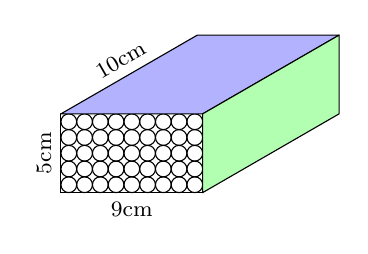
\begin{tikzpicture}[font=\footnotesize,line join=round, line cap=round]
	\def\r{.1}
	\def\g{30}
	\foreach \x in {0,...,8}\foreach \y in {0,...,4}\draw (2*\x *\r ,2*\y *\r) circle (\r);
	\draw
	(-\r,-\r)coordinate (O)--++(0,10*\r)coordinate (A)node[midway,sloped,above]{5cm}
	(O)--++(18*\r,0)coordinate (B)node[midway,sloped,below]{9cm}
	(B)--++(0,10*\r)--(A)
	;
	\draw[fill=blue!30] (A)--++(\g:20*\r)node[midway,sloped,above]{10cm}--++(0:18*\r)--++(\g-180:20*\r)--cycle;
	\draw[fill=green!30](B)--++(\g:20*\r)--++(90:10*\r)--++(\g-180:20*\r)--cycle;
\end{tikzpicture}
\end{document}